\subsection{Lemmas to assist our proof}    
In order to assist our proof, we define two \textit{lemmas} based on the ordering relations. 

\begin{lemma} Consider three events $e$,$d$ and $k$. \\

    If
        \[
            \cons{e}{d} \ \wedge \ \reln{e}{ao}{d} \ \wedge \
            (
                (\et{d}{uo}) \ \vee \
                (\et{d}{sc} \ \wedge \ \event{d}{W})
            )
        \]
        
    then,
        \[
            \reln{k}{hb}{d} \Longrightarrow \reln{k}{hb}{e}
        \]
      
    When we have two consecutive events \textit{e} and \textit{d} which are one after the other (i.e. $\reln{e}{ao}{d}$), we can use \textit{transitive property} of $\stck{_{hb}}$ to infer that any event \textit{k} that \textit{happens before} \textit{e}, also \textit{happens before} \textit{d}. However, is it possible to derive that the event \textit{k happens before e} using the evidence that \textit{k happens before d} ? This lemma states the condition when this is true.
    
\end{lemma}

%An alternative short proof 
\begin{proof}
    
    We will divide the proof for this into two cases, based on what event $d$ is. For both cases, we have the following to be true :
    
    \[
        cons(e,d) \ \wedge \ \reln{e}{ao}{d}
        \tag{0}
        \label{l10}
    \]

    In the first case, 
    
    \[
        \et{d}{uo} 
        \tag{1}
        \label{l11}
    \]
    
    Then for any event $k$
    \[
        dir(k,d) \Rightarrow cons(k,d)
        \qquad from \quad
        (\ref{l11})
        \tag{2}
        \label{l12}
    \]
    
    An event that satisfies the above with $d$ is $e$.
    \[
         k = e  
         \qquad from \quad
         (\ref{l10}, \ref{l12})
         \tag{3}
         \label{l13}
    \]
    
    Because $\stck{_{ao}}$ is a total order, $e$ will be the only event. This would mean that for any other $k \neq e$,
    
    \[
        \reln{k}{hb}{d} \Rightarrow \reln{k}{hb}{d}
        \qquad from \quad
        (\ref{l10}, \ref{l11}, \ref{l12}, \ref{l13}) 
    \]
    
    The following figure should explain this intuition:  
    \begin{figure}[H]
        \centering
        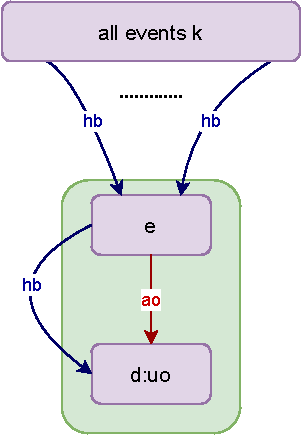
\includegraphics[scale=0.7]{Lemma_Proof1_Case1.pdf}
        \caption{For the first case}
        \label{fig:my_label}
    \end{figure}
    
    In the second case,
    \[
        \et{d}{sc} \wedge d\!\in\!W
        \tag{4}
        \label{l14}
    \]
    
    Then for any event $k$
    \[
        dir(k,d) \Rightarrow cons(k,d)
        \qquad from \quad
        (\ref{l14})
        \tag{5}
        \label{l15}
    \]
    
    We once again have event $e$ satisfying the above
    \[
        k = e 
        \qquad from \quad
        (\ref{l10}, \ref{l15})
        \tag{6}
        \label{l16}
    \]
    
    Though there could be direct \textit{happens-before} relation with some event $k$ from another \textit{agent}, these are only relations satisfying $dir(d,k)$. Thus, we can once again infer that for any $k \neq e$ 
    
    \[
        \reln{k}{hb}{d} \Rightarrow \reln{k}{hb}{d}
        \qquad from \quad
        (\ref{l10}, \ref{l14}, \ref{l15}, \ref{l16})
    \]
    
    The following figure explains this intuition: 
    
    \begin{figure}[H]
        \centering
        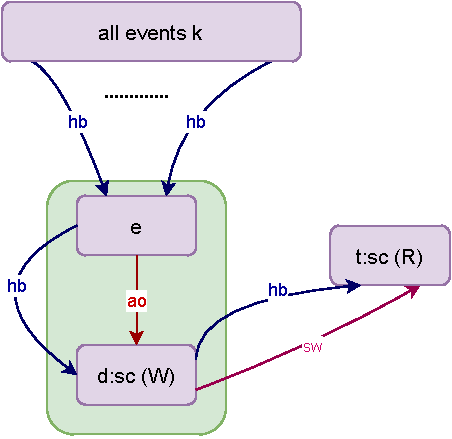
\includegraphics[scale=0.7]{Lemma_Proof1_Case2.pdf}
        \caption{For the second case}
        \label{fig:my_label}
    \end{figure}
    
\end{proof}

%---------------------------------------------------------------------------------------------------------------    

%SHORTER VERSION OF PROOF WITHOUT THE ENGLISH EXPLAINATION IN THE MIDDLE. DISCUSS AND DECIDE ON WHICH FORM IS BETTER
\begin{lemma}Consider three events $e$, $d$ and $k$ \\

    If
        
        \[
            \cons{e}{d} \ \wedge \ \reln{e}{ao}{d} \ \wedge \
            (
                (\et{e}{uo}) \ \vee \
                (\et{e}{sc} \ \wedge \ \event{e}{R})
            )
        \]
        
    then,
        \[
            \reln{e}{hb}{k} \Longrightarrow \reln{d}{hb}{k}
        \]

 When we have two consecutive events \textit{e} and \textit{d} which are one after the other (i.e. $\reln{e}{ao}{d}$), we can use \textit{transitive property} of $\stck{_{hb}}$ to infer that any event \textit{k} that \textit{happens after} \textit{d}, also \textit{happens after} \textit{e}. However, is it possible to derive that the event \textit{k happens after d} using the evidence that \textit{k happens after e} ? This lemma states the condition when this is true.

\end{lemma}

%An alternative proof for this 
\begin{proof}
    
    Just like the proof for the previous lemma, we will divide the proof for this into two cases, based on what event $e$ is. Again, for both cases, we have the following to be true:
    
    \[
        cons(e,d) \ \wedge \reln{e}{ao}{d}
        \tag{0}
        \label{l20}
    \]

   In the first case,
   
   \[
        \et{e}{uo} 
        \tag{1}
        \label{l21}
   \]
   
   Then for any event k
   
   \[
        dir(e,k) \Rightarrow cons(e,k) 
        \qquad from
        \quad (\ref{l21})
        \tag{2}
        \label{l22}
   \]
   
   The event that satisfies the above with $e$ is $d$
   \[
        k = d 
        \qquad from 
        \quad (\ref{l20}, \ref{l22})
        \tag{3}
        \label{l23}
   \]
   
   Because $\stck{_{ao}}$ is a total order, $d$ would be the only such event. This would mean that for any other event $k \neq d$
   
   \[
        \reln{e}{hb}{k} \Rightarrow \reln{d}{hb}{k}
        \qquad from 
        \quad (\ref{l20}, \ref{l21}, \ref{l22}, \ref{l23})
   \]
   %Better phrase the intuition
   The following figure should explain this intuition:  
    
    \begin{figure}[H]
        \centering
        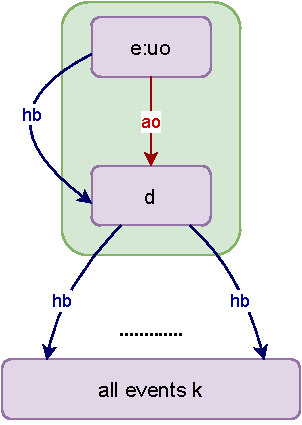
\includegraphics[scale=0.7]{Lemma_Proof2_Case1.pdf}
        \caption{Caption}
        \label{fig:my_label}
    \end{figure}
    
    In the second case,
    \[
        \et{e}{sc} \wedge e\!\in\!R
        \tag{4}
        \label{l24}
    \]
    
    Then for any event $k$
    \[
        dir(e,k) \Rightarrow cons(e,k)
        \qquad from \quad
        (\ref{l24})
        \tag{5}
        \label{l25}
    \]
    
    We once again have event $d$ satisfying the above   
    \[
        k = d 
        \qquad from \quad
        (\ref{l20}, \ref{l25})
        \tag{6}
        \label{l26}
    \]
    
    Though there could be direct \textit{happens-before} relation with some event $k$ from another \textit{agent}, these are only relations satisfying $dir(k,e)$. Thus, we can once again infer that for any $k \neq d$ 
    
    \[
        \reln{e}{hb}{k} \Rightarrow \reln{d}{hb}{k}
        \qquad from \quad
        (\ref{l10}, \ref{l24},  \ref{l25}, \ref{l16})
    \]
    
    The following figure explains this intuition: 
    
    \begin{figure}[H]
        \centering
        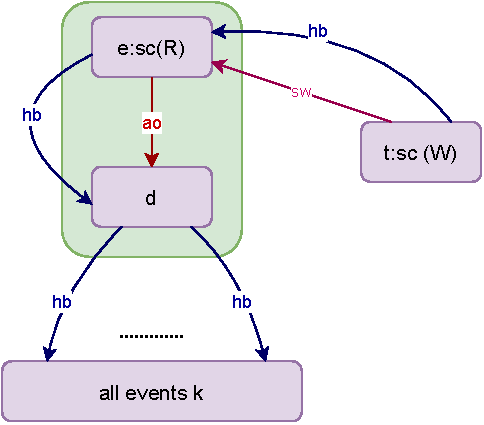
\includegraphics[scale=0.7]{Lemma_Proof2_Case2.pdf}
        \caption{Caption}
        \label{fig:my_label}
    \end{figure}

\end{proof}

%------------------------------------------------------------------------------
